\chapter{Аналитическая часть}

В данном разделе приведена формализация задачи и данных, проанализированы существующие решения, рассмотрены типы пользователей и требуемый функционал. Представлен анализ способов хранения данных, а также произведен выбор оптимального для решения поставленной задачи подхода к хранению данных. 

\section{Формализация задачи}

Необходимо спроектировать и реализовать базу данных для онлайн-мониторинга состояния трасс и подъемников горнолыжного курорта. Также необходимо разработать интерфейс, позволяющий работать с данной базой для получения и изменения хранящейся в ней информации и мониторинга очередей к подъемникам в онлайн-режиме. Требуется реализовать, как минимум, три вида ролей – пользователь, сотрудник лыжного патруля и администратор.

\section{Формализация данных}\label{data}

База данных должна хранить информацию о:
\begin{itemize}
	\item трассах;
	\item подъемниках;
	\item связях трасс и подъемников (на одном подъемнике можно добраться до нескольких трасс, и до одной трассы можно добраться на нескольких подъемниках);
	\item турникетах;
	\item проездных картах;
	\item считываниях карт на турникетах подъемников;
	\item сообщениях о происшествиях;
	\item пользователях;
	\item группах пользователей.
\end{itemize}

В таблице \ref{tbl:1} приведены категории и сведения о данных.

\captionsetup{justification=raggedleft,singlelinecheck=off}
\begin{table}[H]
	\centering
	\caption{Категории и сведения о данных}
	\label{tbl:1}
	\begin{tabular}{|l|l|}
		\hline
		\textbf{Категория}                                                                   & \textbf{Сведения}                                                                                                                                       \\ \hline
		Трассы                                                                               & \begin{tabular}[c]{@{}l@{}}ID трассы, название трассы, уровень\\ сложности, открытость/закрытость.\end{tabular}                                         \\ \hline
		Подъемники                                                                           & \begin{tabular}[c]{@{}l@{}}ID подъемника, название подъемника,\\ открытость/закрытость, количество мест,\\ время подъема, время в очереди.\end{tabular} \\ \hline
		Связи трасс и подъемников                                                            & ID записи, ID подъемника, ID трассы.                                                                                                                    \\ \hline
		Турникеты                                                                            & \begin{tabular}[c]{@{}l@{}}ID турникета, ID подъемника, \\ открытость/закрытость.\end{tabular}                                                          \\ \hline
		Проездные карты                                                                      & ID карты, дата и время активации, тип.                                                                                                                  \\ \hline
		\begin{tabular}[c]{@{}l@{}}Считывания карт на \\ турникетах подъемников\end{tabular} & \begin{tabular}[c]{@{}l@{}}ID записи, ID турникета, ID карты, \\ дата и время считывания.\end{tabular}                                                  \\ \hline
		\begin{tabular}[c]{@{}l@{}}Сообщения о \\ происшествиях\end{tabular}                 & \begin{tabular}[c]{@{}l@{}}ID сообщения, ID отправителя, \\ ID прочитавшего, текст сообщения.\end{tabular}                                              \\ \hline
		Пользователи                                                                         & \begin{tabular}[c]{@{}l@{}}ID пользователя, ID карты, email (логин), \\ пароль, ID группы пользователей.\end{tabular}                                   \\ \hline
		Группы пользователей                                                                 & ID группы пользователей, права доступа.                                                                                                                 \\ \hline
	\end{tabular}
\end{table}

\clearpage
На рисунке \ref{img:er} отображена ER-диаграмма системы, основанная на приведенной выше таблице.


\begin{figure}[h!]
	\begin{center}
		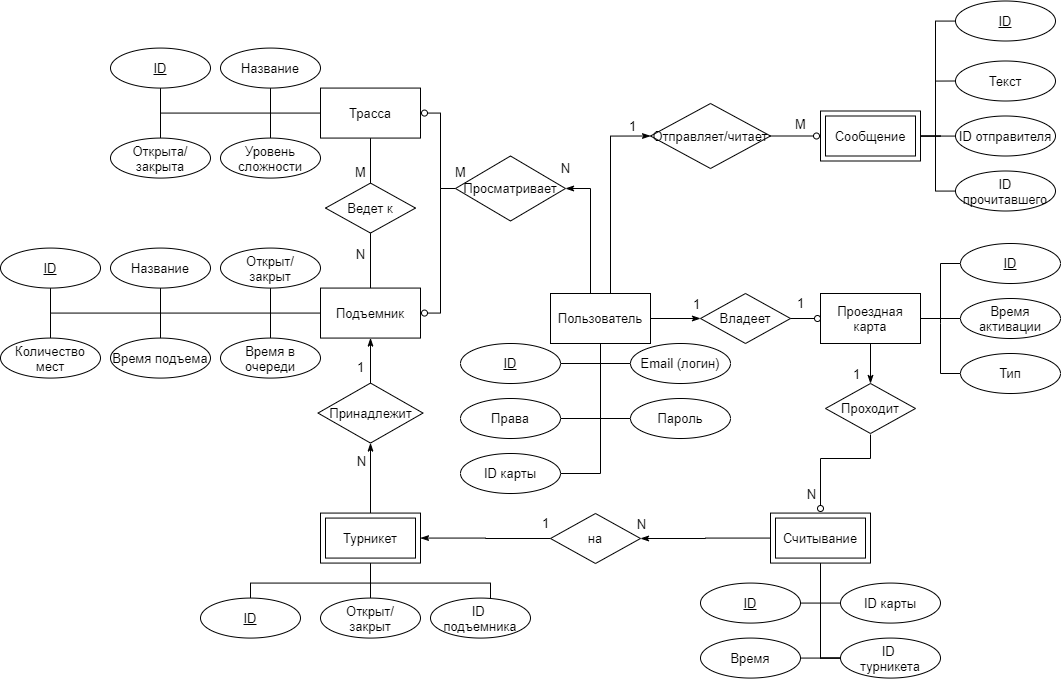
\includegraphics[scale=0.4]{../imgs/er/er_russian.png}
	\end{center}
	\captionsetup{justification=centering}
	\caption{ER-диаграмма}
	\label{img:er}
\end{figure}

\section{Типы пользователей}\label{functions}

В соответствии с поставленной задачей необходимо разработать приложение с возможностью аутентификации пользователей, что делит их, прежде всего, на авторизованных и неавторизованных. Для управления приложением необходима ролевая модель: авторизованный (обычный) пользователь, сотрудник лыжного патруля и администратор. 

Для каждого типа пользователя предусмотрен свой набор функций, который можно описать с помощью текста и Use Case Diagram (диаграммы прецедентов). Она состоит из графической диаграммы, описывающей действующие лица и прецеденты – конкретные действия, которые выполняет пользователь при работе с системой.

\clearpage
Набор функций неавторизованного пользователя:
	\begin{itemize}
		\item регистрация,
		\item аутентификация,
		\item просмотр информации о состоянии трасс и подъемников,
		\item просмотр информации о связях трасс и подъемников.
	\end{itemize}

На рисунке \ref{img:use_case1} представлена диаграмма прецедентов  для неавторизованного пользователя.
\begin{figure}[h!]
	\begin{center}
		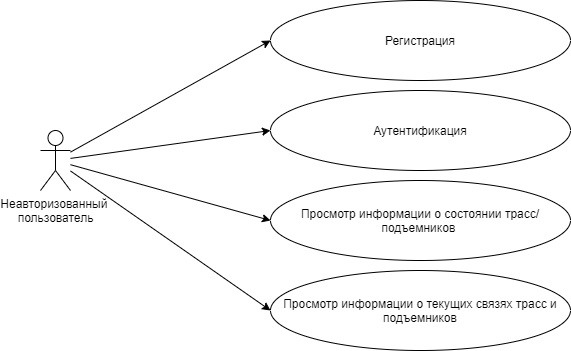
\includegraphics[scale=0.7]{../imgs/use_case/use-case1.png}
	\end{center}
	\captionsetup{justification=centering}
	\caption{Диаграмма прецедентов для неавторизованного пользователя}
	\label{img:use_case1}
\end{figure}
	
	
	
	
	
Набор функций авторизованного пользователя:
	\begin{itemize}
		\item выход,
		\item просмотр информации о состоянии трасс и подъемников,
		\item просмотр информации о связях трасс и подъемников,
		\item отправка сообщений о происшествиях.
	\end{itemize}

\clearpage
На рисунке \ref{img:use_case2} представлена диаграмма прецедентов  для неавторизованного пользователя.

\begin{figure}[h!]
	\begin{center}
		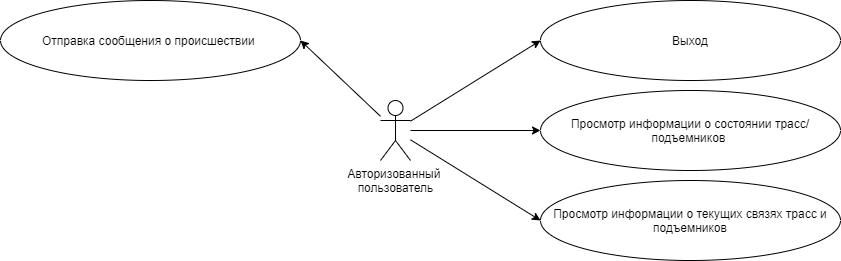
\includegraphics[scale=0.5]{../imgs/use_case/use-case2.png}
	\end{center}
	\captionsetup{justification=centering}
	\caption{Диаграмма прецедентов для авторизованного пользователя\\}
	\label{img:use_case2}
\end{figure}

	
Набор функций сотрудника лыжного патруля:
	\begin{itemize}
		\item выход,
		\item просмотр и изменение информации о состоянии трасс и подъемников,
		\item просмотр и изменение информации о связях трасс и подъемников,
		\item просмотр сообщений о происшествиях.
	\end{itemize}

На рисунке \ref{img:use_case3} представлена диаграмма прецедентов  для сотрудника лыжного патруля.

\begin{figure}[h!]
	\begin{center}
		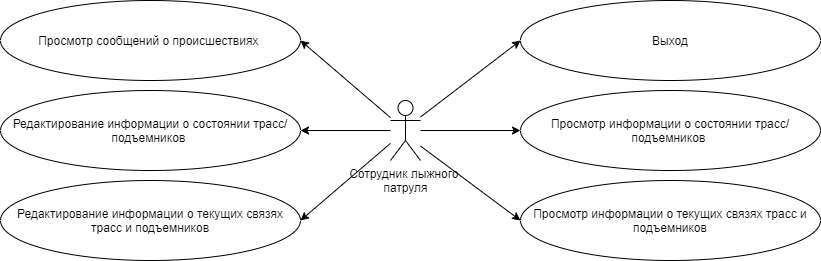
\includegraphics[scale=0.5]{../imgs/use_case/use-case3.png}
	\end{center}
	\captionsetup{justification=centering}
	\caption{Диаграмма прецедентов для сотрудника лыжного патруля}
	\label{img:use_case3}
\end{figure}
	
	
	
\clearpage	
Набор функций администратора:
	\begin{itemize}
		\item выход,
		\item просмотр и изменение всей 
		информации, доступной в базе данных, в том числе права доступа групп и отдельных пользователей.
	\end{itemize}

На рисунке \ref{img:use_case4} представлена диаграмма прецедентов  для администратора.

\begin{figure}[h!]
	\begin{center}
		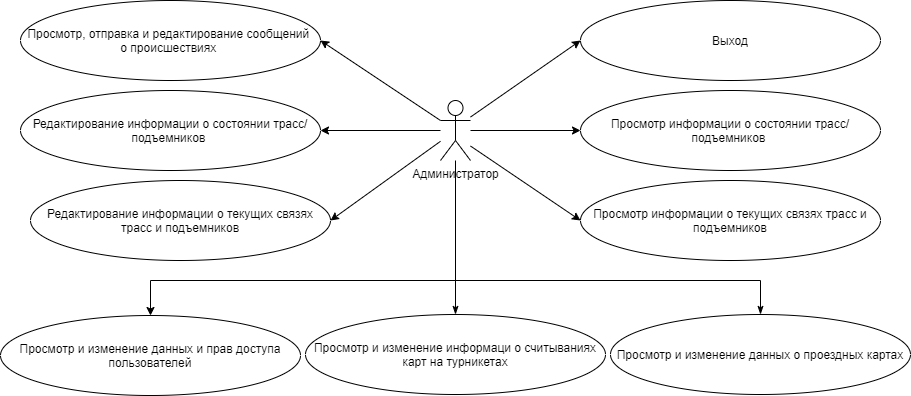
\includegraphics[scale=0.48]{../imgs/use_case/use-case4.png}
	\end{center}
	\captionsetup{justification=centering}
	\caption{Диаграмма прецедентов для администратора}
	\label{img:use_case4}
\end{figure}


\section{Анализ существующих решений}

\subsection{Критерии}\label{criteria}

Проведем анализ аналогичных решений по следующим критериям:
\begin{enumerate}
\item наличие информации об открытости/закрытости трасс и подъемников;
\item наличие информации об очередях на подъемниках; 
\item наличие сводной информации о связях трасс и подъемников;
\item возможность получить информацию о том, до каких трасс можно добраться на конкретном подъемнике/на каких подъемниках можно добраться до конкретной трассы.
\end{enumerate}

\subsection{Мобильное приложение горнолыжного курорта <<Газпром>>}

В приложении горнолыжного курорта <<Газпром>> есть возможность просмотреть информацию об открытости/закрытости трасс (рисунок \ref{img:g}, a) и подъемников (рисунок \ref{img:g}, b), а также сводную информацию о связях трасс и подъемников с помощью карты курорта (рисунок \ref{img:g}, c):

%\clearpage
\begin{figure}[h!]
	\begin{center}
	
	\begin{subfigure}{.33\textwidth}
		\centering
		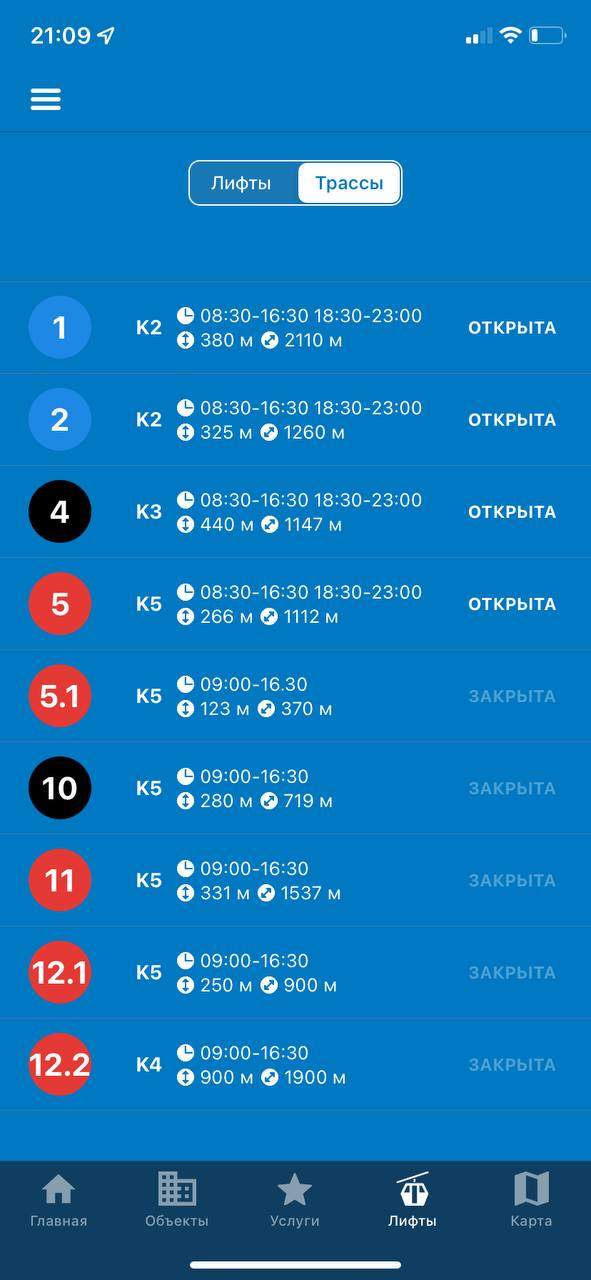
\includegraphics[width=.95\linewidth]{../imgs/analogue_apps/gslope.png}
		\label{img:gslope}
		\captionsetup{justification=centering}
		\caption{}
	\end{subfigure}%
	\begin{subfigure}{.33\textwidth}
		\centering
		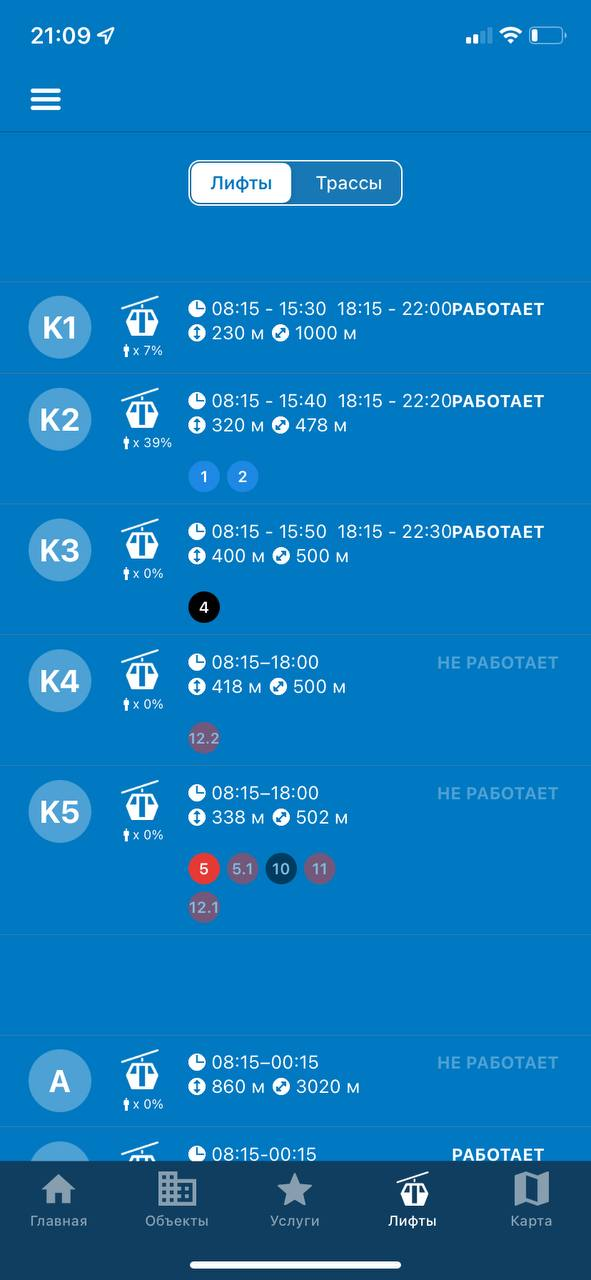
\includegraphics[width=.95\linewidth]{../imgs/analogue_apps/glift.png}
		\label{img:glift}
		\captionsetup{justification=centering}
		\caption{}
	\end{subfigure}%
	\begin{subfigure}{.33\textwidth}
		\centering
		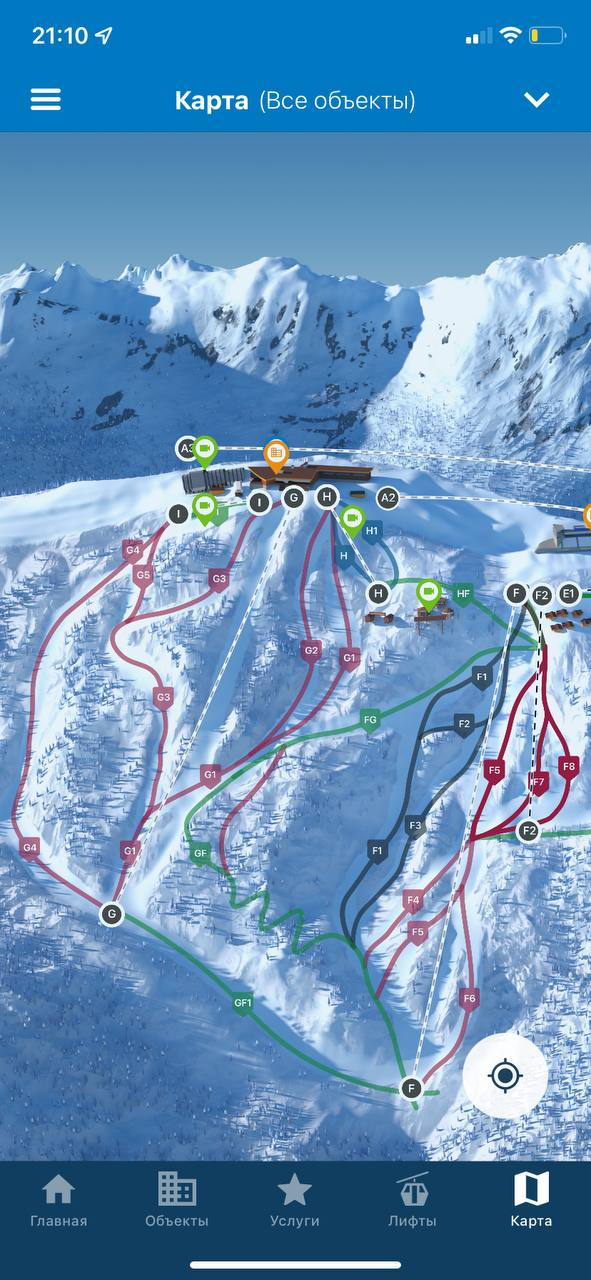
\includegraphics[width=.95\linewidth]{../imgs/analogue_apps/gmap.png}
		\label{img:gmap}
		\captionsetup{justification=centering}
		\caption{}
	\end{subfigure}
	\captionsetup{justification=centering}
	\caption{Просмотр информации в мобильном приложении <<Газпром>>}
	\label{img:g}
	\end{center}
\end{figure}


\clearpage
\subsection{Мобильное приложение курорта <<Courchevel>>}

В приложении горнолыжного курорта <<Courchevel>> на единой карте можно просмотреть информацию об открытости/закрытости трасс и подъемников, а также сводную информацию о связях трасс и подъемников (рисунок \ref{img:Courchevel}):


\begin{figure}[h!]
	\begin{center}
		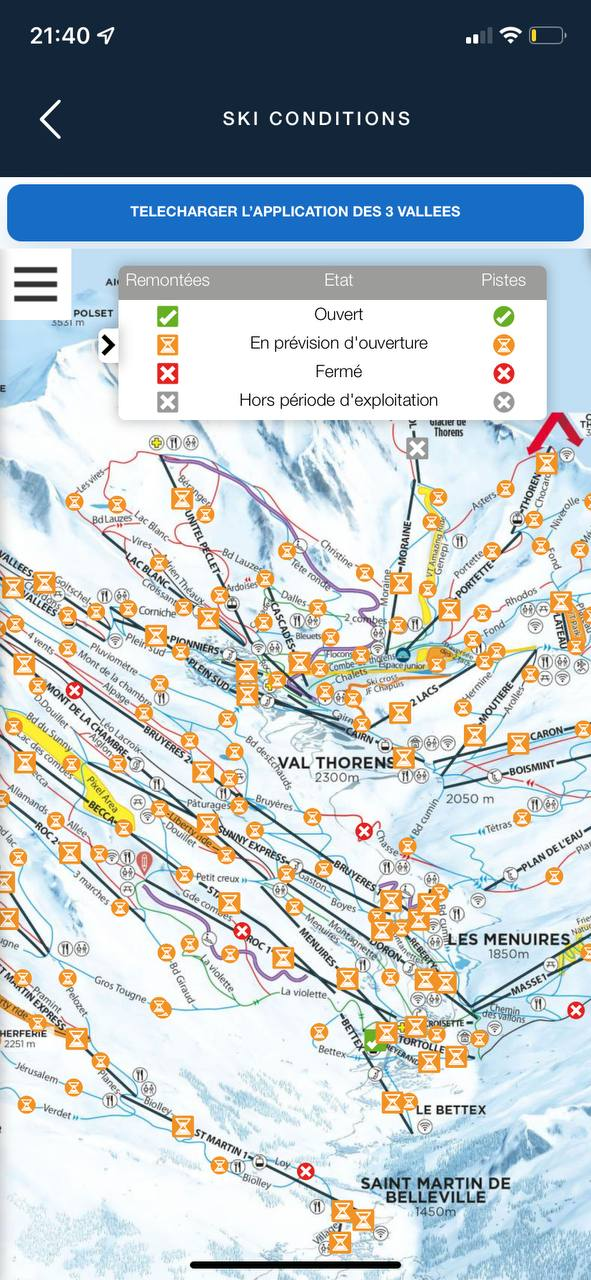
\includegraphics[scale=0.35]{../imgs/analogue_apps/Courchevel.png}
	\end{center}
	\captionsetup{justification=centering}
	\caption{Просмотр информации в приложении <<Courchevel>>}
	\label{img:Courchevel}
\end{figure}


\subsection{Мобильное приложение горнолыжного курорта <<Роза Хутор>>}

В приложении горнолыжного курорта <<Газпром>> есть возможность просмотреть информацию об открытости/закрытости трасс (рисунок \ref{img:r}, a) и подъемников (рисунок \ref{img:r}, b), а также сводную информацию о связях трасс и подъемников с помощью карты курорта (рисунок \ref{img:r}, c):



\begin{figure}[h!]
	\begin{center}
		
		\begin{subfigure}{.33\textwidth}
			\centering
			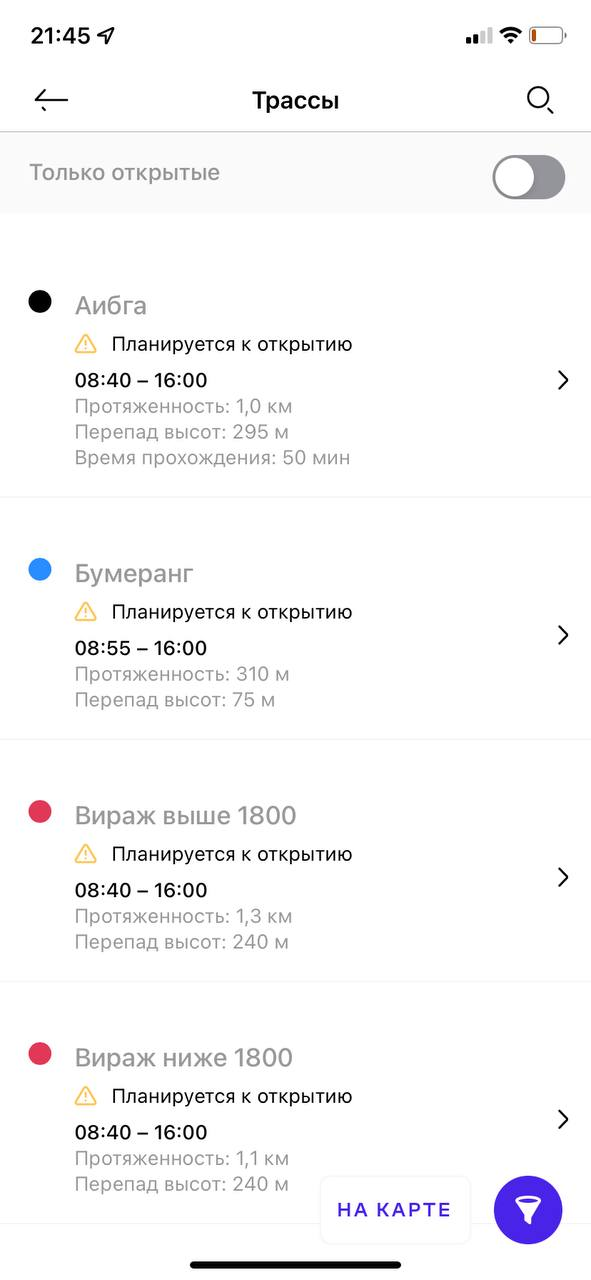
\includegraphics[width=.95\linewidth]{../imgs/analogue_apps/rslope.png}
			\label{img:rslope}
			\captionsetup{justification=centering}
			\caption{}
		\end{subfigure}%
		\begin{subfigure}{.33\textwidth}
			\centering
			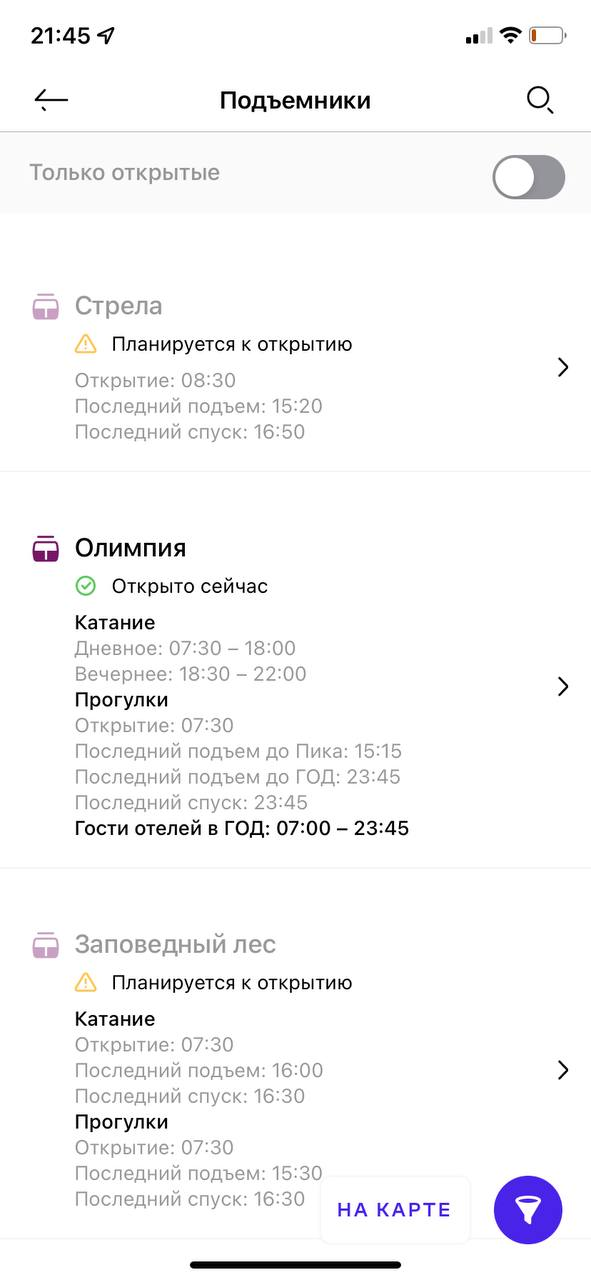
\includegraphics[width=.95\linewidth]{../imgs/analogue_apps/rlift.png}
			\label{img:rlift}
			\captionsetup{justification=centering}
			\caption{}
		\end{subfigure}%
		\begin{subfigure}{.33\textwidth}
			\centering
			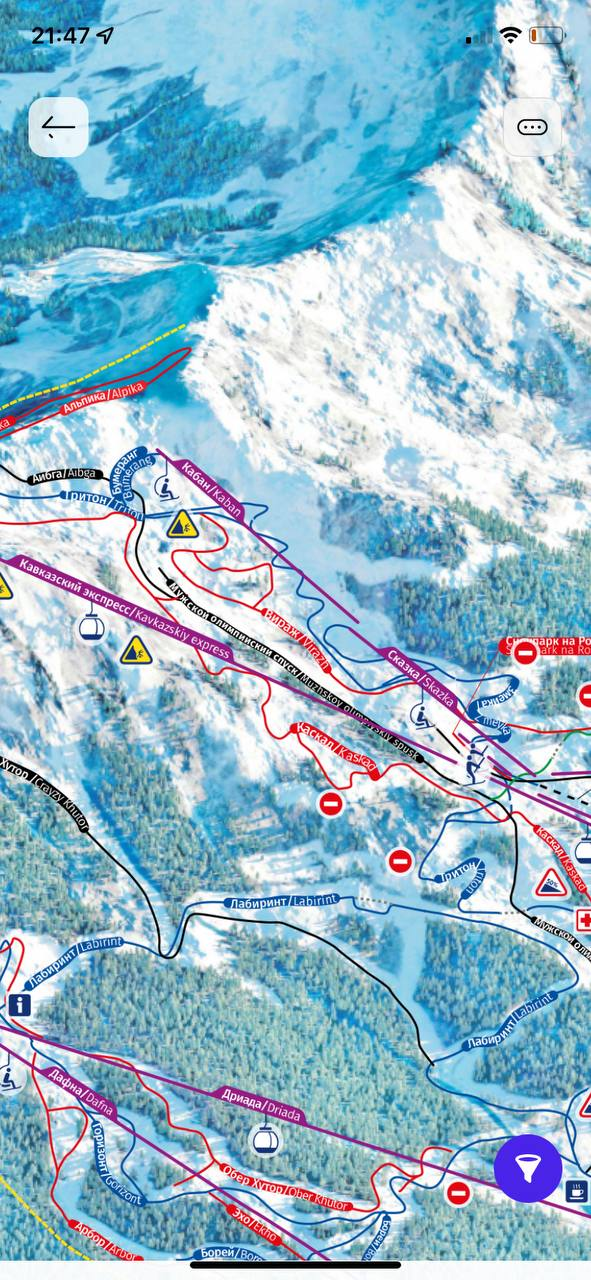
\includegraphics[width=.95\linewidth]{../imgs/analogue_apps/rmap.png}
			\label{img:rmap}
			\captionsetup{justification=centering}
			\caption{}
		\end{subfigure}
		\captionsetup{justification=centering}
		\caption{Просмотр информации в мобильном приложении <<Роза Хутор>>}
		\label{img:r}
	\end{center}
\end{figure}


\clearpage
Также есть возможность в онлайн-режиме просматривать камеры, расположенные на различных объектах курорта (пример показан на рисунке \ref{img:rcamera1}). Этим можно воспользоваться для мониторинга очередей на подъемниках.


\begin{figure}[h!]
	\begin{center}
		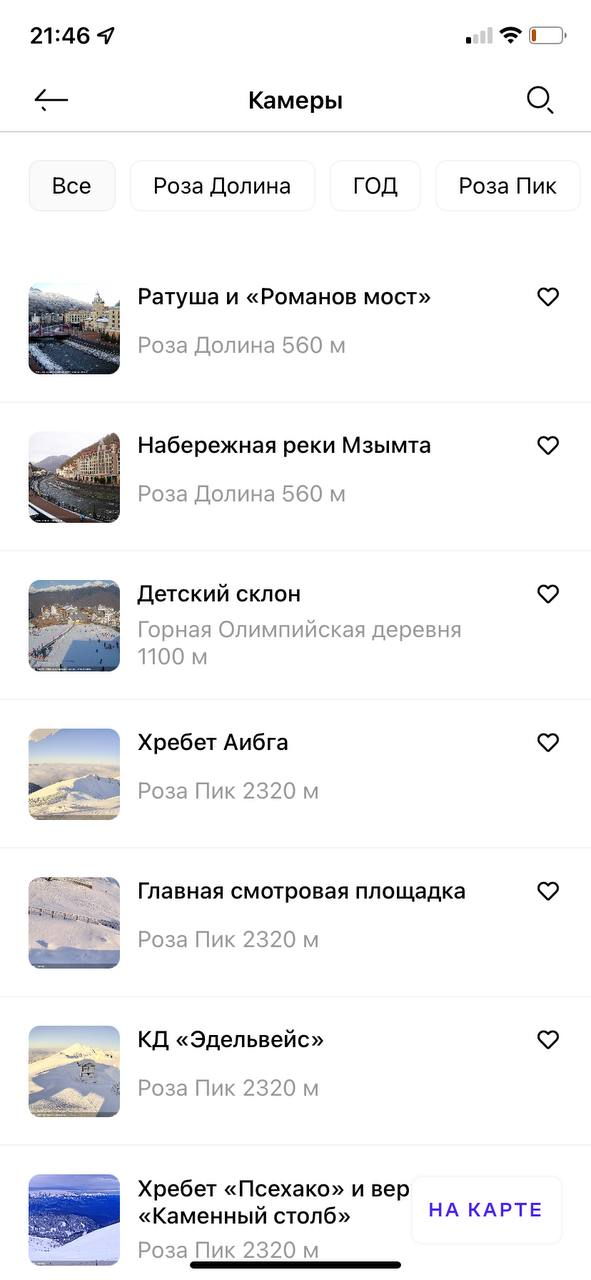
\includegraphics[scale=0.4]{../imgs/analogue_apps/rcamera1.png}
	\end{center}
	\captionsetup{justification=centering}
	\caption{Онлайн-просмотр камер в приложении <<Роза Хутор>>}
	\label{img:rcamera1}
\end{figure}



\subsection{Сравнение существующих решений}

В таблице \ref{tbl:2} приведено сравнение решений по наличию в них информации, перечисленной в пункте \ref{criteria}. В таблице приняты следующие обозначения: открытость -- информация об открытости/закрытости трасс и подъемников, очереди -- информации об очередях на подъемниках, связи (св.) -- сводная информация о связях трасс и подъемников, связи (конкр.) -- информация о связях конкретной трассы с подъемниками или наоборот.

\captionsetup{justification=raggedleft,singlelinecheck=off}
\begin{table}[H]
	\centering
	\caption{Сравнение решений}
	\label{tbl:2}
	\begin{tabular}{|l|l|l|l|l|}
		\hline
		Название & Открытость & Очереди  & Связи (св.) & Связи (конкр.) \\ \hline
		Газпром & + (список) & - & + (на карте) & - \\ \hline
		Courchevel & + (на карте) & - & + (на карте) & - \\ \hline
		Роза Хутор & + (список) & + (камеры) & + (на карте) & - \\ \hline
	\end{tabular}
\end{table}

Таким образом, ни одно из приложений не отображает всю информацию, которую предполагается предоставлять в разрабатываемом приложении. В частности, наименее представлена информация об очередях на подъемниках, которая позволила бы посетителям выбирать мене загруженные объекты и тем самым делать нагрузку более равномерной. Предоставление же информации о том, как добраться до конкретной трассы позволит пользователям (в особенности, новым) упростить организацию своего катания.








\section{Анализ баз данных} 

Для решения поставленной цели необходимо разработать базу данных (БД). БД -- это упорядоченный набор структурированной информации или данных, которые обычно хранятся в электронном виде в компьютерной системе\cite{database}.
%СУБД -- это совокупность программных и лингвистических средств общего или специального назначения, обеспечивающих управление созданием и использованием баз данных

\clearpage
\subsection{Классификация баз данных по месту хранения информации}

По месту хранения информации БД можно разделить на \cite{inmemory}:
\begin{itemize}
	\item традиционные, которые хранят информацию на жестком диске или другом постоянном носителе; 
	\item in-memory databases (IMDB) (резидентные базы данных), которые хранят информацию непосредственно в оперативной памяти.
\end{itemize}

IMDB появились как ответ традиционным БД в связи со снижением стоимости оперативной памяти. Хранение данных в этой области позволяет увеличить скорость их обработки в сотни раз \cite{why}. При этом резидентные БД обеспечивают высокую пропускную способность систем, критичных к производительности \cite{adv}.

Обратной стороной этих достоинств являются следующие недостатки:
\begin{itemize}
	\item однопоточность и эффективная утилизация только одного ядра процессора, что не позволяет в полной мере воспользоваться возможностями современных многоядерных серверов;
	\item энергозависимость и привязка к размеру оперативной памяти.
\end{itemize}

В практическом плане IMDB-системы особенно востребованы в тех приложениях работы с данными в реальном времени, где требуется минимальное время отклика \cite{lookslike}.

\subsection{Выбор БД по месту хранения информации}\label{imdb}
Основным требованием к разрабатываемой БД является предоставление возможности \textbf{онлайн}-мониторинга состояния объектов горнолыжного курорта. Задача предполагает постоянное добавление и изменение данных. С особо высокой частотой будут добавляться считывания карт на турникетах подъемников. При этом время в очереди на подъемник должно регулярно пересчитываться и обновляться, чтобы пользователь не получил устаревшую информацию. Решение также предполагает быструю отзывчивость на запросы пользователя.  

Таким образом, задача является типовым примером использования IMDB. И поскольку в современных in-memory СУБД существуют надежные и достаточно простые способы устранения указанных недостатков этих БД, было принято решение использовать именно этот подход к хранению данных.





\section*{Вывод}
В данном разделе была проведена формализация задачи и данных, проанализированы существующие решения, рассмотрены типы пользователей и требуемый функционал. В результате анализа способов хранения данных, для данной задачи был сделан выбор в пользу резидентной БД.


